\documentclass{standalone}
\usepackage{tikz}
\usetikzlibrary{patterns, positioning}


\begin{document}
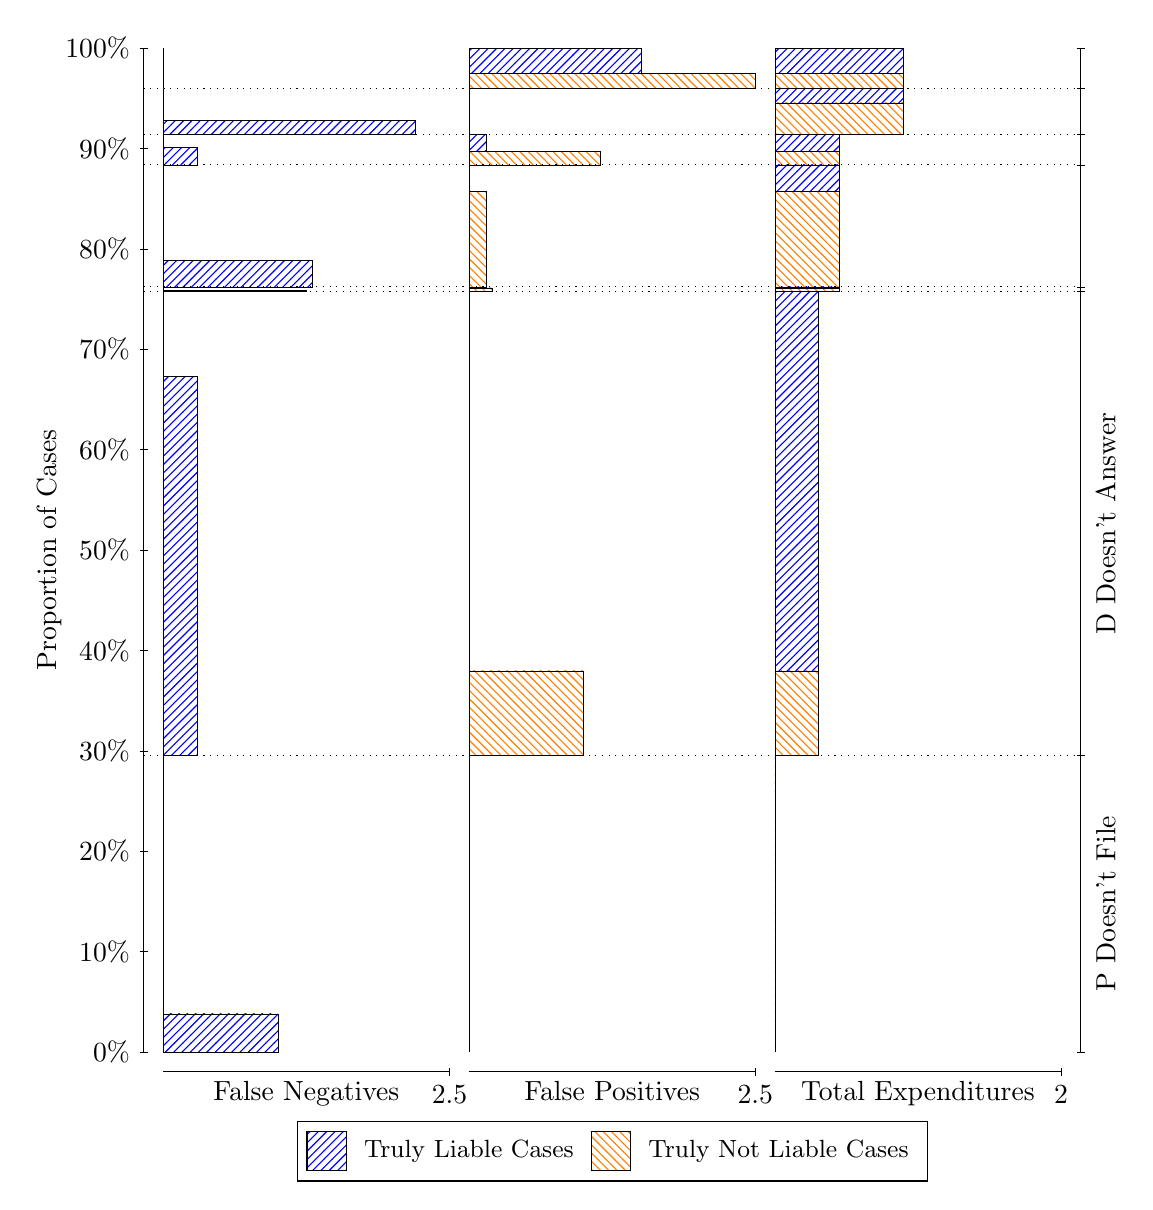
\begin{tikzpicture}
\draw[black, very thin] (1.5,1.75) -- (1.5,14.5);
\node[rotate=90, text=black, anchor=center] at (0.3, 8.125) {Proportion of Cases};
\draw[black, very thin] (1.45,1.75) -- (1.55,1.75);
\node[text=black, anchor=east] at (1.45, 1.75) {0\%};
\draw[black, very thin] (1.45,3.025) -- (1.55,3.025);
\node[text=black, anchor=east] at (1.45, 3.025) {10\%};
\draw[black, very thin] (1.45,4.3) -- (1.55,4.3);
\node[text=black, anchor=east] at (1.45, 4.3) {20\%};
\draw[black, very thin] (1.45,5.575) -- (1.55,5.575);
\node[text=black, anchor=east] at (1.45, 5.575) {30\%};
\draw[black, very thin] (1.45,6.85) -- (1.55,6.85);
\node[text=black, anchor=east] at (1.45, 6.85) {40\%};
\draw[black, very thin] (1.45,8.125) -- (1.55,8.125);
\node[text=black, anchor=east] at (1.45, 8.125) {50\%};
\draw[black, very thin] (1.45,9.4) -- (1.55,9.4);
\node[text=black, anchor=east] at (1.45, 9.4) {60\%};
\draw[black, very thin] (1.45,10.675) -- (1.55,10.675);
\node[text=black, anchor=east] at (1.45, 10.675) {70\%};
\draw[black, very thin] (1.45,11.95) -- (1.55,11.95);
\node[text=black, anchor=east] at (1.45, 11.95) {80\%};
\draw[black, very thin] (1.45,13.225) -- (1.55,13.225);
\node[text=black, anchor=east] at (1.45, 13.225) {90\%};
\draw[black, very thin] (1.45,14.5) -- (1.55,14.5);
\node[text=black, anchor=east] at (1.45, 14.5) {100\%};

\draw[black, very thin] (13.4,1.75) -- (13.4,14.5);
\draw[black, very thin] (13.35,1.75) -- (13.45,1.75);
\node[anchor=west] at (13.35, 1.75) {};
\draw[black, very thin] (13.35,5.5119) -- (13.45,5.5119);
\node[anchor=west] at (13.35, 5.5119) {};
\draw[black, very thin] (13.35,11.407) -- (13.45,11.407);
\node[anchor=west] at (13.35, 11.407) {};
\draw[black, very thin] (13.35,11.466) -- (13.45,11.466);
\node[anchor=west] at (13.35, 11.466) {};
\draw[black, very thin] (13.35,13.016) -- (13.45,13.016);
\node[anchor=west] at (13.35, 13.016) {};
\draw[black, very thin] (13.35,13.401) -- (13.45,13.401);
\node[anchor=west] at (13.35, 13.401) {};
\draw[black, very thin] (13.35,13.989) -- (13.45,13.989);
\node[anchor=west] at (13.35, 13.989) {};
\draw[black, very thin] (13.35,14.5) -- (13.45,14.5);
\node[anchor=west] at (13.35, 14.5) {};

\draw[black, very thin, pattern color=blue, pattern=north east lines] (1.75,1.75) rectangle (3.2033,2.2345);
\draw[black, very thin, pattern color=orange, pattern=north west lines] (1.75,2.2345) rectangle (1.75,5.5119);
\draw[black, very thin, pattern color=blue, pattern=north east lines] (1.75,5.5119) rectangle (2.186,10.33);
\draw[black, very thin, pattern color=orange, pattern=north west lines] (1.75,10.33) rectangle (1.75,11.407);
\draw[black, very thin, pattern color=blue, pattern=north east lines] (1.75,11.407) rectangle (3.5667,11.418);
\draw[black, very thin, pattern color=orange, pattern=north west lines] (1.75,11.418) rectangle (1.75,11.466);
\draw[black, very thin, pattern color=blue, pattern=north east lines] (1.75,11.466) rectangle (3.6393,11.799);
\draw[black, very thin, pattern color=orange, pattern=north west lines] (1.75,11.799) rectangle (1.75,13.016);
\draw[black, very thin, pattern color=blue, pattern=north east lines] (1.75,13.016) rectangle (2.186,13.234);
\draw[black, very thin, pattern color=orange, pattern=north west lines] (1.75,13.234) rectangle (1.75,13.401);
\draw[black, very thin, pattern color=blue, pattern=north east lines] (1.75,13.401) rectangle (4.9473,13.585);
\draw[black, very thin, pattern color=orange, pattern=north west lines] (1.75,13.585) rectangle (1.75,13.989);
\draw[black, very thin, pattern color=orange, pattern=north west lines] (1.75,13.989) rectangle (1.75,14.173);
\draw[black, very thin, pattern color=blue, pattern=north east lines] (1.75,14.173) rectangle (1.75,14.5);
\draw[black, very thin, pattern color=orange, pattern=north west lines] (5.6333,1.75) rectangle (5.6333,5.0274);
\draw[black, very thin, pattern color=blue, pattern=north east lines] (5.6333,5.0274) rectangle (5.6333,5.5119);
\draw[black, very thin, pattern color=orange, pattern=north west lines] (5.6333,5.5119) rectangle (7.0867,6.589);
\draw[black, very thin, pattern color=blue, pattern=north east lines] (5.6333,6.589) rectangle (5.6333,11.407);
\draw[black, very thin, pattern color=orange, pattern=north west lines] (5.6333,11.407) rectangle (5.924,11.455);
\draw[black, very thin, pattern color=blue, pattern=north east lines] (5.6333,11.455) rectangle (5.6333,11.466);
\draw[black, very thin, pattern color=orange, pattern=north west lines] (5.6333,11.466) rectangle (5.8513,12.684);
\draw[black, very thin, pattern color=blue, pattern=north east lines] (5.6333,12.684) rectangle (5.6333,13.016);
\draw[black, very thin, pattern color=orange, pattern=north west lines] (5.6333,13.016) rectangle (7.3047,13.183);
\draw[black, very thin, pattern color=blue, pattern=north east lines] (5.6333,13.183) rectangle (5.8513,13.401);
\draw[black, very thin, pattern color=orange, pattern=north west lines] (5.6333,13.401) rectangle (5.6333,13.804);
\draw[black, very thin, pattern color=blue, pattern=north east lines] (5.6333,13.804) rectangle (5.6333,13.989);
\draw[black, very thin, pattern color=orange, pattern=north west lines] (5.6333,13.989) rectangle (9.2667,14.173);
\draw[black, very thin, pattern color=blue, pattern=north east lines] (5.6333,14.173) rectangle (7.8133,14.5);
\draw[black, very thin, pattern color=orange, pattern=north west lines] (9.5167,1.75) rectangle (9.5167,5.0274);
\draw[black, very thin, pattern color=blue, pattern=north east lines] (9.5167,5.0274) rectangle (9.5167,5.5119);
\draw[black, very thin, pattern color=orange, pattern=north west lines] (9.5167,5.5119) rectangle (10.062,6.589);
\draw[black, very thin, pattern color=blue, pattern=north east lines] (9.5167,6.589) rectangle (10.062,11.407);
\draw[black, very thin, pattern color=orange, pattern=north west lines] (9.5167,11.407) rectangle (10.334,11.455);
\draw[black, very thin, pattern color=blue, pattern=north east lines] (9.5167,11.455) rectangle (10.334,11.466);
\draw[black, very thin, pattern color=orange, pattern=north west lines] (9.5167,11.466) rectangle (10.334,12.684);
\draw[black, very thin, pattern color=blue, pattern=north east lines] (9.5167,12.684) rectangle (10.334,13.016);
\draw[black, very thin, pattern color=orange, pattern=north west lines] (9.5167,13.016) rectangle (10.334,13.183);
\draw[black, very thin, pattern color=blue, pattern=north east lines] (9.5167,13.183) rectangle (10.334,13.401);
\draw[black, very thin, pattern color=orange, pattern=north west lines] (9.5167,13.401) rectangle (11.152,13.804);
\draw[black, very thin, pattern color=blue, pattern=north east lines] (9.5167,13.804) rectangle (11.152,13.989);
\draw[black, very thin, pattern color=orange, pattern=north west lines] (9.5167,13.989) rectangle (11.152,14.173);
\draw[black, very thin, pattern color=blue, pattern=north east lines] (9.5167,14.173) rectangle (11.152,14.5);
\draw[black, dotted] (1.5,5.5119) -- (13.4,5.5119);
\draw[black, dotted] (1.5,11.407) -- (13.4,11.407);
\draw[black, dotted] (1.5,11.466) -- (13.4,11.466);
\draw[black, dotted] (1.5,13.016) -- (13.4,13.016);
\draw[black, dotted] (1.5,13.401) -- (13.4,13.401);
\draw[black, dotted] (1.5,13.989) -- (13.4,13.989);
\draw[black, very thin] (1.75,1.5) -- (5.3833,1.5);
\node[text=black, anchor=north] at (3.5667, 1.5) {False Negatives};
\draw[black, very thin] (5.3833,1.45) -- (5.3833,1.55);
\node[text=black, anchor=north] at (5.3833, 1.45) {2.5};

\draw[black, very thin] (5.6333,1.5) -- (9.2667,1.5);
\node[text=black, anchor=north] at (7.45, 1.5) {False Positives};
\draw[black, very thin] (9.2667,1.45) -- (9.2667,1.55);
\node[text=black, anchor=north] at (9.2667, 1.45) {2.5};

\draw[black, very thin] (9.5167,1.5) -- (13.15,1.5);
\node[text=black, anchor=north] at (11.333, 1.5) {Total Expenditures};
\draw[black, very thin] (13.15,1.45) -- (13.15,1.55);
\node[text=black, anchor=north] at (13.15, 1.45) {2};

\node[text=black, centered, rotate=90] at (13.72, 3.6309) {P Doesn't File};
\node[text=black, centered, rotate=90] at (13.72, 8.4597) {D Doesn't Answer};






\draw (7.449999999999999,1.5) node[draw=none] (baseCoordinate) {};
\begin{scope}[align=center]
        \matrix[scale=0.5, draw=black, below=0.5cm of baseCoordinate, nodes={draw}, column sep=0.1cm]{
            \node[rectangle, draw, minimum width=0.5cm, minimum height=0.5cm, pattern color=blue, pattern=north east lines] {}; &
            \node[draw=none, font=\small, text=black] (B) {Truly Liable Cases}; &
            \node[rectangle, draw, minimum width=0.5cm, minimum height=0.5cm, pattern color=orange, pattern=north west lines] {}; &
            \node[draw=none, font=\small, text=black] (B) {Truly Not Liable Cases}; \\
            };
\end{scope}

\end{tikzpicture}
\end{document}